\documentclass{article}

\usepackage[utf8]{inputenc}
\usepackage[brazilian]{babel}
\usepackage{graphicx}
\usepackage{float}
\usepackage[pdftex]{hyperref}
\usepackage{epstopdf}
\usepackage{etoolbox}
\usepackage{amsmath}
\usepackage{amsfonts}
\usepackage{amssymb}
\usepackage{caption}
\usepackage{subcaption}
\usepackage{setspace}
\usepackage{tikz}

\patchcmd{\thebibliography}{\section*}{\section}{}{}
\newcommand{\R}{\ensuremath{\mathbb{R}}}
\newcommand{\Prob}{\ensuremath{\mathbb{P}}}
\newcommand{\K}{\ensuremath{\mathbb{K}}}
\newcommand{\U}{\ensuremath{\mathbb{U}}}
\newcommand{\N}{\ensuremath{\mathbb{N}}}
\newcommand{\Lg}{\ensuremath{\mathbb{L}}}
\newcommand{\T}{\ensuremath{\rm Tr}}
\newcommand{\sg}{{\sigma(x_k)}}

\newcommand{\G}{\ensuremath{\mathcal{G}}}
\newcommand{\F}{\ensuremath{\mathcal{F}}}
\newcommand{\C}{\ensuremath{\mathcal{C}}}
\newcommand{\E}{\ensuremath{\mathcal{E}}}
\newcommand{\Hn}{\ensuremath{\mathcal{H}}}
%\newcommand{\Hoo}{\ensuremath{\mathcal{H}_\infty}}
\newcommand{\Hop}{\ensuremath{\mathcal{H}_{op}}}
% --------------------------------------------------
\newtheorem{theo}{Teorema}
\newtheorem{exa}{Exemplo}
\newtheorem{lemm}{Lema}
\newtheorem{coro}{Corolário}
\newtheorem{defn}{Definição}[section]

%opening


\begin{document}
\input{capa.tex}

\onehalfspacing
\section{Objetivos} 
O objetivo desse experimento é a identificação da função de transferência de sistemas eletrônicos de terceira ordem. Nesse pré relatório nós iremos estudar um circuito eletrônico, identificar sua função de transferência e com o auxílio do $Matlab$ simular sua resposta. 
	
\section{Análise Do Circuito}
Consideramos o sistema de terceira ordem que pode ser representado pelo circuito apresentado na figura \ref{fig:circuito}, cujos parâmetros numéricos estão na tabela \ref{tab:valores}.

\begin{figure}[H]
\centering
\includegraphics[width=0.7\linewidth]{CircuitoPlanta}
\caption{Esquema do sistema de terceira ordem$^{\cite{bb:roteiro}}$}
\label{fig:circuito}
\end{figure}

\begin{table}[H]
\centering
\caption{Resistência e capacitância dos componentes}
\label{tab:valores}
\begin{tabular}{|c|c|}
	\hline Componente & Valor \\ 
	\hline $R_1$ & $100$ [$K\Omega$] \\ 
	\hline $R_2$ & $10$ [$K\Omega$] \\ 
	\hline $R_3$ & $100$ [$K\Omega$] \\ 
	\hline $R_4$ & $220$ [$K\Omega$] \\ 
	\hline $R_5$ & $100$ [$K\Omega$] \\ 
	\hline $R_6$ & $470$ [$K\Omega$] \\ 
	\hline $R_7$ & $1$ [$M\Omega$] \\ 	
	\hline $C_1$ & $0,1$ [$\mu F$] \\ 	
	\hline $C_2$ & $0,1$ [$\mu F$] \\ 	
	\hline $C_3$ & $0,1$ [$\mu F$] \\ 	
	\hline 
\end{tabular} 
\end{table}

\subsection{Determinação da Função de Transferência de cada Estágio}
Através das ferramentas tradicionais de equacionamento de circuitos, sabemos que para um elemento como representado na figura \ref{fig:unidade} teremos:

\begin{figure}[H]
\centering
\includegraphics[width=0.3\linewidth]{unidade}
\caption{Circuito Integrador com limitação do ganho em dc}
\label{fig:unidade}
\end{figure}
 
\begin{equation}
I = \frac{V_{in}}{R_a}
\end{equation}
\begin{equation}
V_{out} = \frac{-I}{\frac{1}{R_b} + Cs}
\end{equation}

Logo, para um módulo desses, teremos:
\begin{equation}
\label{eq:ampop}
G(s) = \frac{V_{out}}{V_{in}} = \frac{-\frac{R_b}{R_a}}{R_bCs + 1}
\end{equation}

Utilizando a equação \ref{eq:ampop} podemos obter as funções de transferência para o estágio 1 fazendo $C=0$, $R_a=R_1$ e $R_b=R_2$. E para os 2 e 3 fazemos as substituições diretas. No estágio 4 faremos a análise direta pela impedância equivalente para obter sua função de transferência, dessa maneira obtemos:

\begin{equation}
\label{eq:ft1}
G_1(s) = -\frac{R_2}{R_1}
\end{equation}
\begin{equation}
\label{eq:ft2}
G_2(s) = \frac{-\frac{R_4}{R_3}}{R_4C_1s + 1}
\end{equation}
\begin{equation}
\label{eq:ft3}
G_3(s) = \frac{-\frac{R_6}{R_5}}{R_6C_2s + 1}
\end{equation}
\begin{equation}
\label{eq:ft4}
G_4(s) = -\frac{1}{R_7C_3s}
\end{equation}

Substituindo os valores numéricos:
\begin{equation}
\label{eq:ftn1}
G_1(s) = -0.1
\end{equation}
\begin{equation}
\label{eq:ftn2}
G_2(s) = \frac{-2.2}{0.022s + 1}
\end{equation}
\begin{equation}
\label{eq:ftn3}
G_3(s) = \frac{-4.7}{0.047s + 1}
\end{equation}
\begin{equation}
\label{eq:ftn4}
G_4(s) = -\frac{10}{s}
\end{equation}
\subsection{Determinação da Função de Transferência do Sistemas}
Sabendo as funções de transferência de cada estágio, a função de transferência do sistema pode ser escrita como o produto destas. Logo, usando as equações \ref{eq:ftn1},\ref{eq:ftn2},\ref{eq:ftn3} e \ref{eq:ftn4} obtemos:
\begin{equation}
\label{eq:ftsistema}
G(s) = G_1(s)G_2(s)G_3(s)G_4(s) = \frac{10340}{1.034s^3 + 69s^2 + 1000s}
\end{equation}

\subsection{Diagrama de Bode e Margens de Fase e Ganho}
Com o auxílio do $Matlab$ plotamos o diagrama de Bode para o sistema e calculamos suas margens de ganho e de fase, que podem ser vistas na figura \ref{fig:bode}. O sistema é estável em malha fechada e tem margem de ganho de $16.2dB$ e margem de fase de $54,9^o$.
\begin{figure}[H]
\centering
\includegraphics[width=0.8\linewidth]{bode}
\caption{Diagrama de Bode do sistema com margens de ganho e de fase}
\label{fig:bode}
\end{figure}
\subsection{Resposta à onda quadrada}
Por fim, analisamos a resposta em cada estágio do sistema a uma onda quadrada de frequência $1Hz$ e amplitude $1Volt$ aplicada em $r$. Com o auxílio do $Matlab$ plotamos essas respostas que podem ser vistas na figura \ref{fig:resposta}
\begin{figure}[H]
\centering
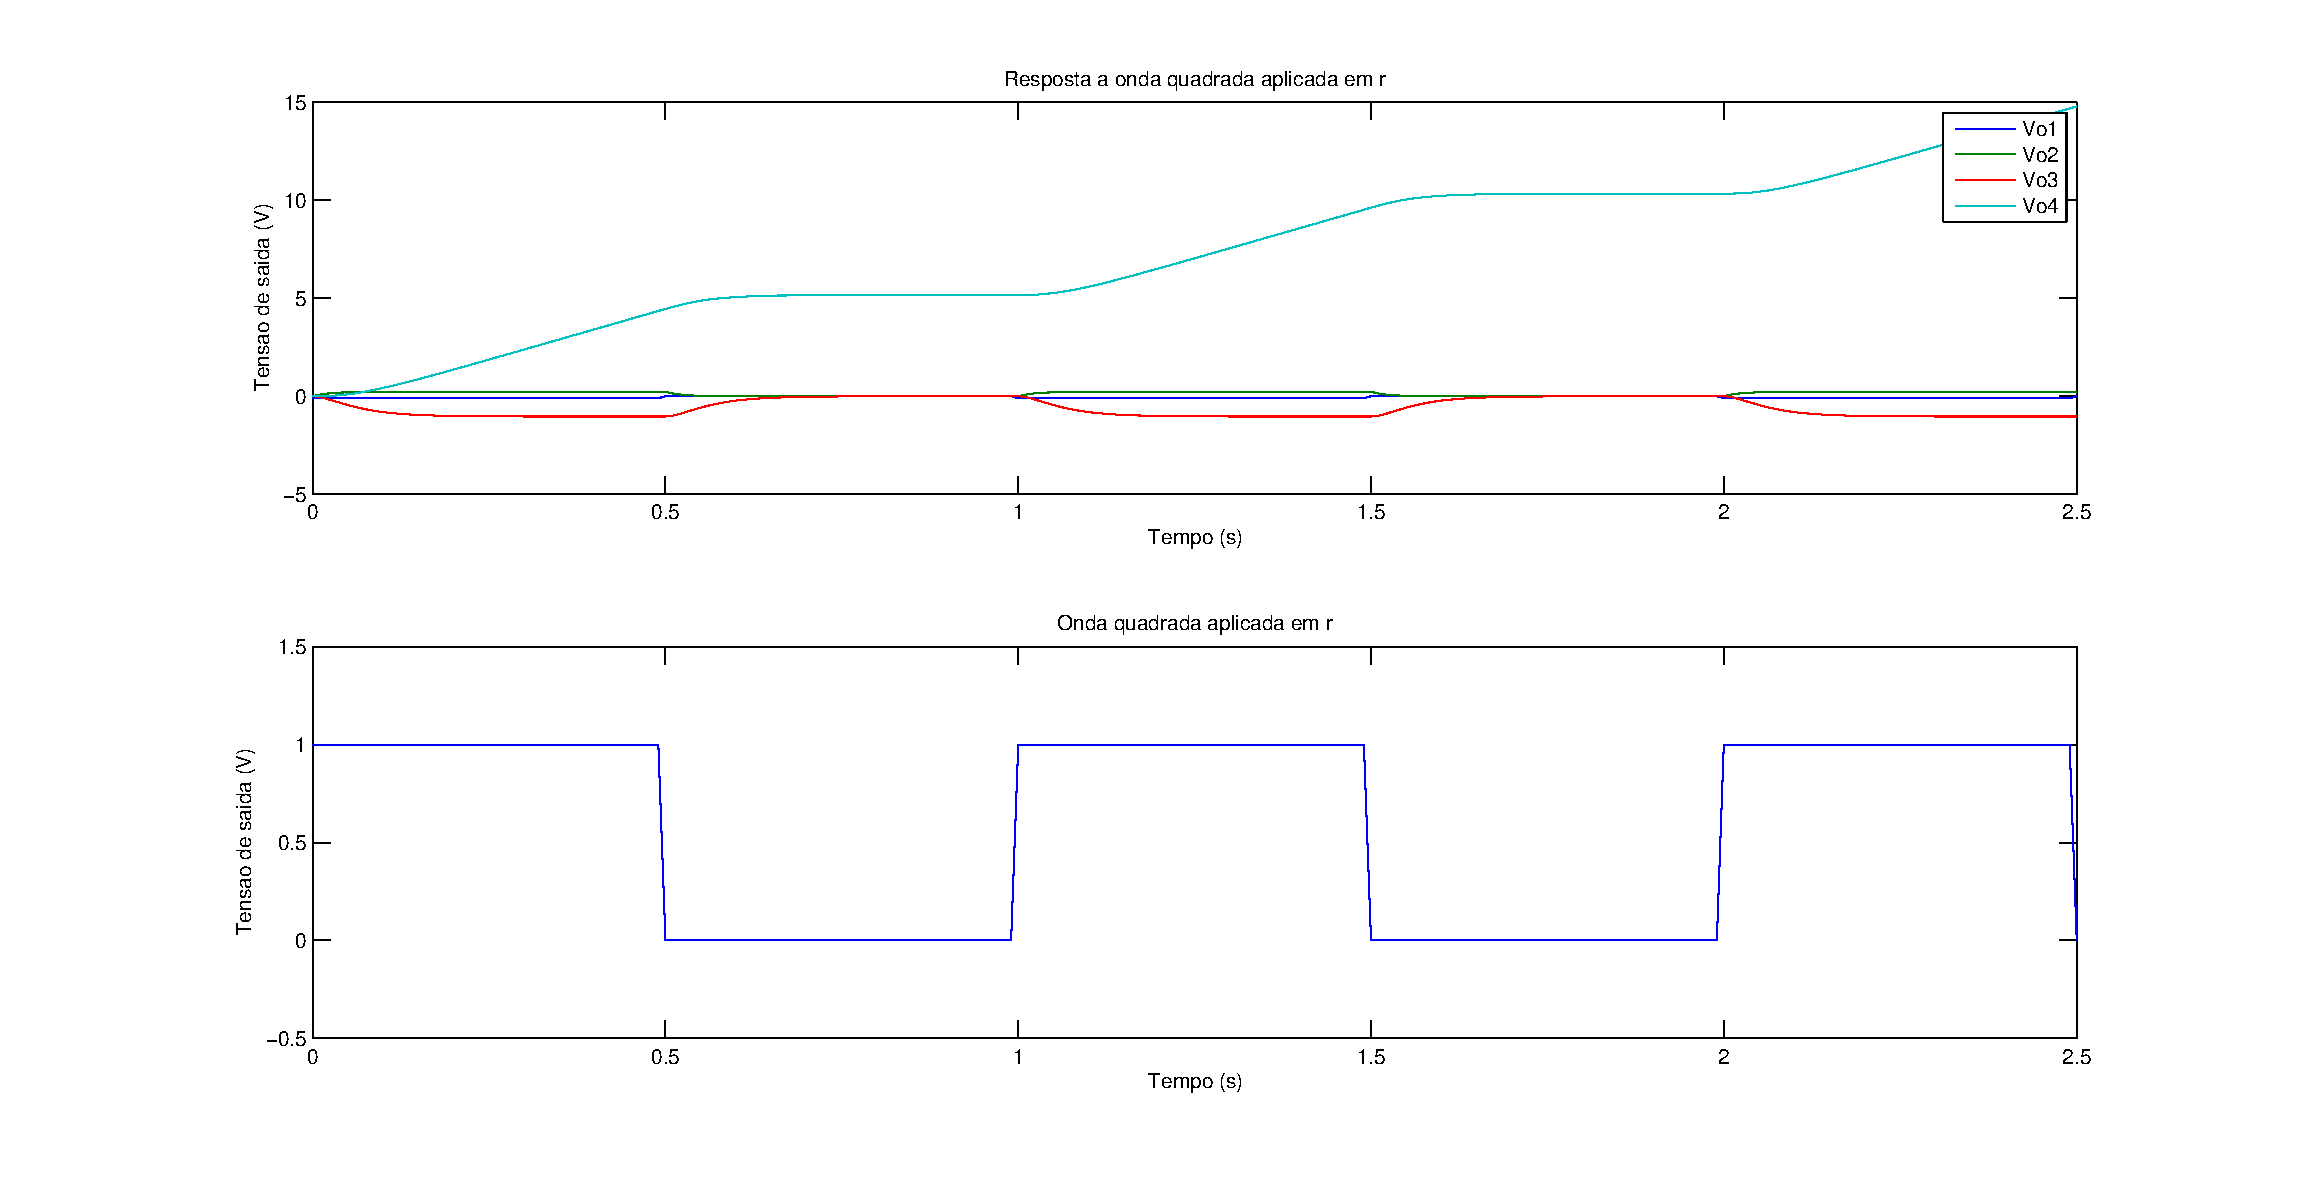
\includegraphics[width=\linewidth, height=0.8\linewidth]{resposta}
\caption{Resposta em cada estágio à uma onda quadrada}
\label{fig:resposta}
\end{figure}

\begin{thebibliography}{widestlabel}
	\bibitem{bb:roteiro}{Roteiro do experimento disponibilizado para os alunos}
\end{thebibliography}
\tiny{Este documento foi formatado utilizando \LaTeX}
\end{document}

